\documentclass[9pt]{sig-alternate-05-2015}

\usepackage{url}
\usepackage{epsfig}
%\usepackage[TABBOTCAP]{subfigure}
\usepackage{tabularx}
\usepackage{graphicx}
\graphicspath{ {images/} }
\usepackage{color}
\usepackage{xspace}
\usepackage{listings}
\usepackage{fancyvrb}
\usepackage{booktabs}
\usepackage{colortbl}
\usepackage{mathtools}
\usepackage{paralist}

\setlength{\paperheight}{11in}
\setlength{\paperwidth}{8.5in}
\setlength{\textwidth}{7in}
\setlength{\textheight}{9.25in}
\setlength{\oddsidemargin}{-.25in}
\setlength{\evensidemargin}{-.25in}
%\setlength{\headsep}{0in}
%\pagenumbering{arabic}

\renewcommand{\paragraph}[1]{{\bf #1}}

\begin{document}

\conferenceinfo{ANCS 2016} {}
\CopyrightYear{2015}
\crdata{X}
\date{}

\CopyrightYear{2016} 
\setcopyright{acmlicensed}
\conferenceinfo{ANCS '16,}{March 17 - 18, 2016, Santa Clara, CA, USA}
\isbn{978-1-4503-4183-7/16/03}\acmPrice{\$15.00}
\doi{http://dx.doi.org/10.1145/2881025.2881030}

%%%%%%%%%%%% THIS IS WHERE WE PUT IN THE TITLE AND AUTHORS %%%%%%%%%%%%

\title{Is Memory Disaggregation Feasible?\\A Case Study with Spark SQL}

\author{Pramon Biligiri and George Porter\\UC San Diego}

\maketitle

%\thispagestyle{empty}

%%%%%%%%%%%%%  ABSTRACT GOES HERE %%%%%%%%%%%%%%
\subsection*{Abstract}

This paper explores the feasibility of disaggregated memory from compute and
storage for a particular, widely deployed workload, Spark
SQL~\cite{Armbrust:2015:SSR:2723372.2742797} analytics queries.  We measure the
empirical rate at which records are processed and calculate the effective
memory bandwidth utilized based on the sizes of the columns accessed in the
query.  Our findings contradict conventional wisdom: not only is memory
disaggregation possible under this workload, but achievable with already
available, commercial network technology.  Beyond this finding, we also
recommend changes that can be made to Spark SQL to improve its ability to
support memory disaggregation.

\section{Introduction}

Achieving efficiency in data processing requires balanced computing, meaning
that a system has the right mix of CPU, memory, storage IO, and network IO so
that one part of the computation is not bottlenecked waiting for results from
another part of the computation.  Getting this balance just right is a moving
target, since the input data, number and type of queries, presence of failures,
and network conditions are in a constant state of flux.  Correctly provisioning
bare-metal servers is a challenge since one must determine their specific
configuration at entirely the wrong timescales, well before they are put into
production.  While virtual machines play an important role in providing more
flexibility in balancing resources, they are not enough.  Even with VMs, you are
limited to configurations implementable in a single server, you are subject to
``fragmentation'' of resources, and you are not able to
upgrade individual components like CPU and memory independently of each other.

These challenges have led to disaggregated server designs, where individual
components such as CPU, memory, and storage are interconnected over a network,
rather than over a bus within a single
chassis~\cite{Han:2013:NSR:2535771.2535778}.  The advantages of disaggregation
include more efficient utilization of resources, and the ability to
independently upgrade different system components.  The challenge for
disaggregation is the ``memory wall''~\cite{Wulf:1995:HMW:216585.216588}. Today
storage is commonly disaggregated via SANs and other network-based file storage
protocols, and Facebook has introduced a disaggregated system-\-on-\-chip (SoC)
platform called Yosemite~\cite{fb-yosemite}, which relies on networked storage.
Yet there is a growing gap in the rate at which CPUs can execute instructions
and the rate at which data can be fetched into the CPU from main memory.  For
this reason in Yosemite (as well as other designs), memory and CPU are still
tightly integrated in the same chassis.

This paper puts aside the issue of disaggregating memory in general, and
instead examines disaggregating memory for a common and increasingly deployed
type of application: analytics queries. Using Spark
SQL~\cite{Armbrust:2015:SSR:2723372.2742797} as a motivating platform, we
measure the actual rate at which threads of execution access memory and process
records, and using these measurements, determine the feasibility of
disaggregating memory.

Our initial results show that even after significant optimization, Spark SQL
analytics queries access memory an order of magnitude slower than the
underlying components permit, opening up the possibility of disaggregating
memory from compute.  In fact, the requirements on the underlying network are
modest, and can be met with existing commercial products such as 40- and
100-Gb/s NICs (e.g., the Mellanox ConnectX-4 NIC~\cite{mellanox100g}).  We
conclude by recommending further changes that improve Spark SQL's ability to
support memory disaggregation.

\section{Motivation}

A major reason that server disaggregation attempts have avoided memory is that,
at a component level, the bandwidth required between memory and the CPU is too
large to be supported by commercial network equipment. We demonstrate this
experimentally in microbenchmark in Section~\ref{sec:memory_wall}.  Yet users
do not run microbenchmarks, they run applications, which might not have such
stringent requirements.  We explore one such application in
Section~\ref{sec:sparksql}, chosen because of its highly efficient use of
memory, serving as a compelling motivating application.

\subsection{The memory wall: barrier or paper tiger?}
\label{sec:memory_wall}

\begin{figure}
\centering
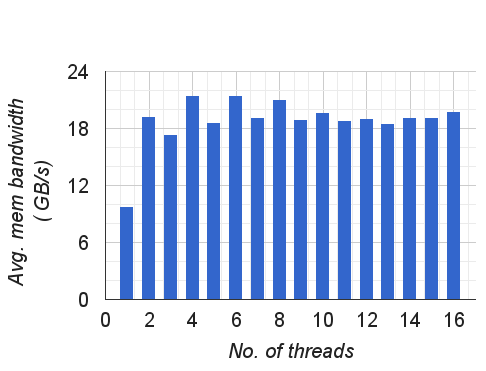
\includegraphics[width=\columnwidth]{stream-bandwidth}
\caption{\label{fig:stream}Aggregate memory bandwidth of STREAM benchmark}
\end{figure}

We start by examining an upper-bound on the bandwidth requirements of a memory
disaggregated system through the STREAM benchmark~\cite{mccalpin1995stream},
which is a synthetic benchmark that measures sustainable memory bandwidth and
the corresponding computation rate for simple vector kernels. A wrapper tool
called stream-scaling~\cite{streamScaling} automates the process of executing
STREAM over the various core counts is used in this study.  We have deployed
STREAM onto an 8-core Intel Xeon 2.27 GHz E5520 processor-based HP ProLiant
DL380 G6 server.  This machine has 24GB of DDR3 Synchronous RAM (1333 MHz),
configured as 12x2GB banks in the Advanced Error Correction Code mode.

Figure~\ref{fig:stream} shows the results of the STREAM Copy benchmark on the
experiment hardware, which copies data from one array of doubles to another.
The total memory bandwidth of the system with all cores active is approximately
21 GB/sec (or 168 Gb/s), a result that matches the HP ProLiant
datasheet~\cite{hpProliant}.  Not only does 168 Gb/s exceed any commercially
available network interface card (NIC), it exceeds the PCIe 3.0 bandwidth
capacity (a x16 device is limited to 15.75 GB/s), meaning that modern servers
are simply unable to keep up with such demand.  Thus, absent additional
constraints, memory disaggregation is not feasible.  We now consider this
problem when constrained to a specific, though popular and widely deployed,
application.

\subsection{Analytic queries with Spark SQL}
\label{sec:sparksql}

Spark SQL~\cite{Armbrust:2015:SSR:2723372.2742797} is a relational data
processing system implemented in Scala and built on top of the functional
programming API of Apache Spark~\cite{Zaharia:2010:SCC:1863103.1863113}. It
bridges the gap between traditional analytics queries and machine
learning algorithms by offering both an SQL interface and a procedural
programmatic interface.

Analytics queries are used to generate summary reports from large amounts of
raw data in order to glean insights. They are characterized by: (1) accessing
the source data in a read-only manner, (2) accessing a large number of rows
from a table (frequently the entire table), but only for a small subset of all
the available columns in the table, (3) performing aggregation operations
(count, sum, average, group by) on one or more columns or tables, and (4)
consisting of CPU-intensive operations for advanced analytics and machine
learning algorithms.  To this last point, Ousterhout et
al.~\cite{Ousterhout:2015:MSP:2789770.2789791} have shown that for a large set
of realistic workloads, Spark is CPU-bound, not memory, network, or storage
bound.  Due to the nature of aggregation-based queries, the size of the working
set can decrease, in some cases significantly, after every stage of
aggregation.

In this paper, we chose Spark SQL due to its highly-efficient use of memory,
due in part to two major factors: (1) it stores data in a column oriented
format, making it efficient to access all the rows of a column, and (2) it
generates Java bytecode directly for commonly used aggregation operations like
{\em count}, {\em min}, and {\em max}, thus avoiding the overhead of multiple,
and possibly virtual, function calls.  We deploy a series of analytic queries
taken from the literature and published benchmarks, and for each thread of
execution, we measure the rate at which records are processed and calculate the
effective memory bandwidth based on the sizes of the columns accessed in the
query multiplied by the number of threads.  This results in the overall
aggregate memory bandwidth.

Specifically, if there are {\em threadcount} threads accessing {\em size} bytes
from each record, during a time interval of $AvgTime_{100000}$ between every
100,000 records (averaged across all the threads), the aggregate memory access
rate is:

\begin{equation}
Mem\_access\_rate =  \frac{(size \times 100000)}{AvgTime_{100000}} \times threadCount
\label{eqn:membw}
\end{equation}

We use this formula to calculate the actual memory access rate, rather than
potential access rate, for sets of queries.

\subsection{High-speed networking}

Today 10- and 40-Gb/s Ethernet is commercially available and widely deployed
within production data centers~\cite{fb-dc}.  Commercial 100 Gb/s NICs and
switches are now available from vendors such as Mellanox~\cite{mellanox100g}.
Already 400 Gb/s Ethernet is in the standardization
process~\cite{ethernet400g}, and terabit standards are on the
horizon~\cite{terabitethernet}.  A key aspect of these new standards is that
their high overall speeds are obtained by joining multiple, parallel,
underlying links together.  For example, 100 Gb/s Ethernet is largely 4 25 Gb/s
lanes, and 400 Gb/s is currently 16 25 Gb/s lanes (eventually to be replaced
with 4 100 Gb/s lanes when those become available).  Simply put, the ability to
increase a single lane of Ethernet cannot keep pace with overall bandwidth
demands, and so parallelism is used in new standards.  As we will see, these
parallel lanes match well to multi-core systems.

\section{Experimental setup}

\subsection{Hardware and software}

The hardware used for the following experiments is a cluster of five nodes,
consisting of a single master node and four workers. Each server is the same
configuration as described above in Section~\ref{sec:memory_wall}, and they are
interconnected with a 10 Gb/s network.  Our measurement methodology ensures
that this network is not a bottleneck for profiling the bandwidth requirements
of the memory system, as described below.

We use Apache Spark 1.3.0~\cite{sparkUrl}, deployed in standalone mode on
Ubuntu Linux 14.04.2.  One executor process is run on each worker node and is
allotted 18GB of RAM out of the 24GB. To read CSV files, we use the spark-csv
library~\cite{sparkCsv}. The Java Virtual Machine used is Java HotSpot
1.6.0\_45-b06.  No other software is running on this cluster apart from the
default system processes.

\subsection{Spark SQL}

Apart from allocating ample memory (18 GB) to each node, we have set up Spark
in a way that increases the demand on the memory subsystem compared to more
general configurations, in an effort to provide a conservative upper-bound on
the memory bandwidth requirements.  Unless mentioned as follows, we maintain
the default Spark configuration~\cite{sparkConfig}.  We have modified
the following settings:

\begin{enumerate}

\item We ensure all memory accesses are to local memory.  In production
workloads, off-node memory might be accessed as well.

\item {\it spark.storage.memoryFraction} is increased to 0.8 (default: 0.6).
This is the fraction of Java heap to use for Spark's memory cache; increasing
this value ensures that resilient distributed datasets (RDDs) are cached
entirely in memory.

\item We set {\it spark.shuffle.spill} to false. This ensures that data does
not spill over to disk during the reduce phase.

\item Memory compression is turned off ({\it
spark.sql.\-inMemory\-Columnar\-Storage.\-compressed}) to reduce extra overhead
on the CPU during query processing.

\item Our instrumentation measures access times after every 100,000 records,
and so we set {\it spark.sql.\-inMemory\-Columnar\-Storage\-.batch\-Size} to
100001 (from its default of 1000) to ensure we have a sufficient number of
records in each batch.

\item We turn on dynamic code generation ({\it
spark.\-sql.\-code\-gen}).  This optimization within Spark SQL
generates Scala code at runtime which is specialized for the types and the
number of expressions used in the query. It also avoids autoboxing overhead
where primitive types are being used. In the absence of code generation, simple
operations like extracting a column from a row, or adding two literals, can
result in branching and virtual function calls. The code generation feature
generates inline Scala code for the same and compiles them to JVM bytecode
before execution.

\item To prevent Spark from writing data to disk during the shuffle phase, we
ensure intermediate data is written to memory by setting the partition to a
{\it tmpfs} filesystem~\cite{WikiTmpfs}.

\item We disable the OS swap partition (via {\it swapoff -a}).

\item Whenever measurements are needed for a specific number of threads, we
achieve that by splitting up the data into an equivalent number of RDD
partitions. The flags used for this are
{\it spark.hadoop.\-fs.local.\-block.\-size} and
{\it spark.hadoop.mapreduce.\-input.file\-input\-format.\-split.minsize}.

\end{enumerate}

\subsection{Workloads}
\label{sec:workloads}

We evaluate the feasibility of memory disaggregation using three workloads.
The first is the STREAM benchmark, described previously, which measures the raw
capacity of the memory subsystem, setting the upper bound on what application
could obtain.  The second is a microbenchmark of Spark SQL's memory access
performance, achieved by measured a simple {\it COUNT(1)} query, which simply
scans a synthetic RDD with rows and columns of different lengths, using a
varying number of threads, all while incrementing a counter.  This sets an
upper-bound on the performance of Spark SQL, as it forms one of the simplest
queries possible to express.
Third, we evaluate a series of more complex queries drawn from the UC Berkeley
AMPLab ``Big Data'' benchmark~\cite{bigDataBenchmark}.

\subsection{Measurement technique}
\label{sec:measurement}

We measure memory bandwidth at the application level by instrumenting Spark
SQL, and validate these measurements by comparing to CPU-level performance
counters.

\paragraph{Spark SQL instrumentation:} Spark SQL loads data into an in-memory
table accessed via the {\it InMemoryColumnarTableScan} class. Data for all rows
of a column is stored in a Java byte array. The first 4 bytes of the array are
used to specify the data type, and the rest contain the actual data.  We
request that the data for the query be cached in memory through Spark's {\it
rdd.persist()} mechanism.  When the query is executed for the first time, a CSV
file is read to populate the in-memory table; subsequent executions of the
query access only the in-memory representation.  We log timing information
within {\it InMemoryColumnarTableScan} during iterations over the table, at
intervals of 100,000 records in each of the threads. Equation~\ref{eqn:membw}
is used to calculate the access rate to memory.  All measurements are taken at
one of the worker nodes in the cluster.

\paragraph{CPU performance counters:} Intel processors provide a set of
counters and associated monitoring software~\cite{intelPerf} to measure CPU
utilization and bytes read/written from memory.  We use these during query
processing to validate the application-level measurements, and our findings
(not shown) match those reported by the Spark-level instrumentation.

\section{Experimental results}

We examine the memory demands of analytical queries first by examining a
trivial query that provides an upper-bound on the bandwidth that can be
achieved by Spark SQL, and then by considering two more complex queries drawn
from the AMPLab's Big Data Benchmark~\cite{amplab_benchmark}.

\subsection{Microbenchmark queries}

\begin{Verbatim}[frame=single,label=Query 1]
SELECT COUNT(1) from SingleColumnTable;
\end{Verbatim}

\begin{figure}[h]
\centering
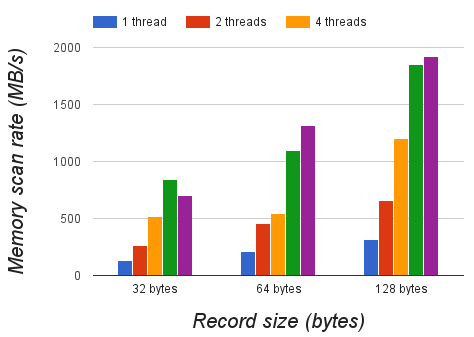
\includegraphics[width=\columnwidth]{mem-scan-rates}
\caption{\label{fig:count1}{\it Select count(1)} query}
\end{figure}

Spark SQL implements Query 1 by fetching the data from the smallest column in
the row and then incrementing a counter. If the row contains only one column,
this is equivalent to fetching the entire row. We chose Query 1 as an example
of a query with minimum CPU usage in order to measure baseline performance of
the system.  Based on the time taken to count every 100,000 records, the memory
access rate is calculated according to Equation~\ref{eqn:membw}.

Columns of data, of various lengths, were generated and mapped to different
numbers of partitions in order to create the appropriate number of threads.
Figure~\ref{fig:count1} shows that a maximum average throughput of 1.9 GB/sec
is seen when running with 16 threads on 128 bytes of data, all from the
in-memory cache. While the throughput increases with the number of threads, it
tapers off as it reaches 16 threads. Since the hardware has only 16-cores,
running more than 16 threads is not representative of the CPU intensive nature
of analytics queries.

\begin{figure}[h]
\centering
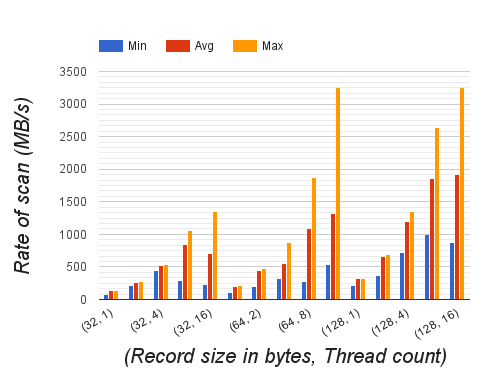
\includegraphics[width=\columnwidth]{mem-scan-summary-statistics}
\caption{\label{fig:stat_query1}Summary statistics for Query 1}
\end{figure}

Figure~\ref{fig:stat_query1} shows the average, max and minimum rates of memory
access for Query 1. It can be seen that a maximum throughput of 1.9 GB/sec is
observed while scanning records of size 64 bytes in 16 threads.  The key
takeaway from this result is that while under optimal conditions, Spark SQL is
capable of driving, in aggregate, an impressive 15 Gb/s of network bandwidth on
our hardware, it requires 16 independent threads to do so.  Each of these
threads, individually, is only capable of sustaining 0.94 Gb/s on average

\begin{figure}[h]
\centering
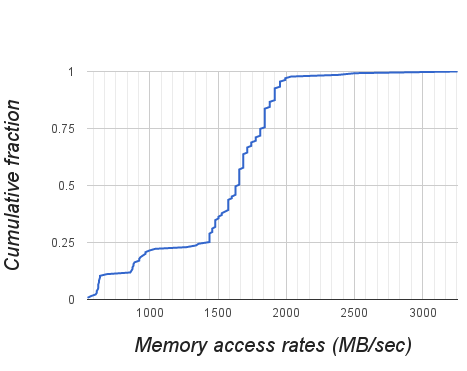
\includegraphics[width=\columnwidth]{cdf-mem-access-rates-count-64bytes-16threads}
\caption{\label{fig:mem_query1}CDF of memory access rates for Query 1 (60M records, 64 bytes, 16 threads)}
\end{figure}

\begin{figure}[h]
\centering
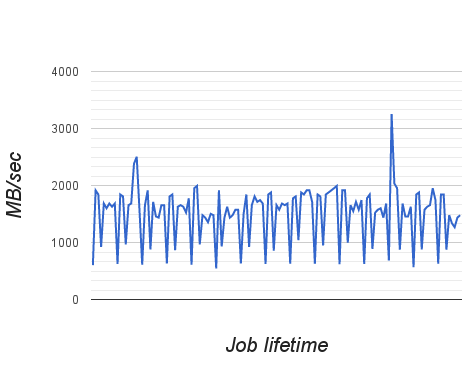
\includegraphics[width=\columnwidth]{time-mem-access-rates-count-64bytes-16threads.png}
\caption{\label{fig:memrate}Memory access rates over job lifetime for Query 1 (60M records, 64 bytes, 16 threads)}
\end{figure}

\subsection{AMPLab Benchmark queries}

The previous section has looked at microbenchmark queries, which are
significantly memory-intensive, and found that they are satisfiable with 40 or
100 Gb/s Ethernet devices currently available from vendors such as
Mellanox~\cite{mellanox100g}.  We now turn our attention to more realistic
queries, provided by the AMPLab ``Big Data'' benchmark
suite~\cite{amplab_benchmark}.

\subsubsection{``Group by'' query}

\begin{Verbatim}[frame=single,label=Query 2]
SELECT sourceIp, SUM(adRevenue) FROM
 uservisits GROUP BY sourceIp
\end{Verbatim}

We next look at an Aggregation Query from the Big Data Benchmark
\cite{bigDataBenchmark}, shown as Query 2.  It shows the advertisement revenue
obtained from each end user IP address based on all the sites visited by that
IP address and grouping  the total revenue obtained from each of those
addresses.  The {\em uservisits} table has 10 million entries. For each row,
the following columns are accessed: sourceIp and adRevenue.
Table~\ref{tbl:data_query2} shows that the data accessed per row of this query
is 23 bytes.

\begin{table}
\begin{tabular}[c]{|l|c|c|}
 \hline
 Column name & Column size & Comments \\
 \hline
 sourceIp & 19 bytes & 4 byte length; 15 byte IP \\ \hline
 adRevenue & 4 bytes & sizeof(FLOAT)\\
 \hline
 Total & 23 bytes & \\
 \hline
\end{tabular}
\caption{\label{tbl:data_query2}Data accessed per row for Query 2}
\end{table}

Spark SQL creates 8 threads to process this data on each node.  The data
accessed per row is 23 bytes, and the average time interval between every
100,000 records is $63.7$ ms, and the minimum is $51.0$ ms.  Based on
Equation~\ref{eqn:membw}, this translates to an access rate of $289$ MB/s (2.3
Gb/s), and a maximum rate of $361$ MB/s (2.9 Gb/s).  Per thread, however, the
demands are a relatively paltry 289 Mb/s on average, 361 Mb/s max.

\begin{figure}
\centering
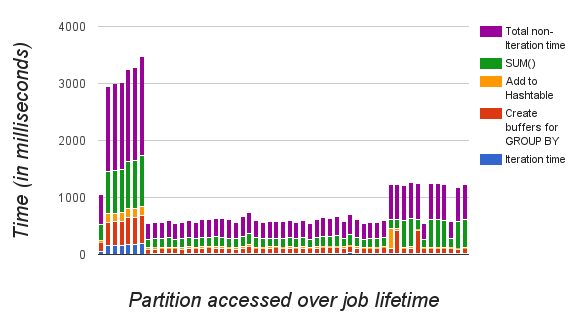
\includegraphics[width=\columnwidth]{group-by-without-codegen}
\caption{\label{fig:codegen}Code generation optimizes memory access rates for Query 2}
\end{figure}

\paragraph{Effect of code generation:} Since Query 2 is more resource intensive
(in terms of both CPU and memory) than Query 1, it is instructive to look at
the performance of the query without bytecode generation.
Figure~\ref{fig:codegen} shows the time spent in various phases of Query 2 in
the absence of code generation. Due to the creation of a large number of
temporary helper objects for aggregation, and the accompanying garbage
collections, the time spent for iterating over data is larger than needed,
showing that to get high memory utilization, it is essential to run with code
generation enabled.  Even with this optimization, it is still practical to
support this result with existing network technology.

\subsubsection{``Join'' query}

\begin{small}
\begin{Verbatim}[frame=single,label=Query 3]
SELECT sourceIp, AVG(pageRank) as avgPageRank,
  SUM(adRevenue) as totalRevenue 
          FROM 
              Rankings AS R, Uservisits AS UV 
         WHERE 
             R.pageUrl = UV.destinationUrl AND 
            UV.visitDate > '1980-01-01' AND 
            UV.visitDate < '2015-05-20' 
         GROUP BY 
             UV.sourceIp 
        ORDER BY totalRevenue DESC LIMIT 1
\end{Verbatim}
\end{small}

We next examine a {\em join} query taken from the Big Data Benchmark
\cite{bigDataBenchmark}, shown here as Query 3. Along with the advertisement
revenue obtained from each end user IP address, it also displays the average
rank of the pages visited by that IP address, by joining with a Rankings table.
The Uservisits table has 10 million rows as earlier, and the Rankings query
also has 10 million rows.  To analyze this query it is necessary to inspect the
in memory representation more closely (shown in Tables~\ref{tbl:query3a} and
\ref{tbl:query3b}). Since the data for Rankings is split into 2 partitions on
the given node and the data for Uservisits is split into 7 partitions, the
number of threads operating upon the two tables are also respectively 2 and 7.
        
\begin{table}
\begin{tabular}[c]{|l|c|c|}
\hline
Column name & Column size & Comments \\
\hline
url & 59 bytes & 4 byte length; 55 bytes data \\
\hline
pageRank & 4 bytes & sizeof(FLOAT) \\
\hline
Total & 63 bytes & \\
\hline
\end{tabular}
\caption{\label{tbl:query3a}Data accessed per row for Query 3 (Rankings table)}
\end{table}

\begin{table}
\begin{tabular}[c]{|l|c|c|}
 \hline
 Column name & Column size & Comments \\
 \hline
 adRevenue & 4 bytes & sizeof(FLOAT) \\
 destinationUrl & 59 bytes & 4 byte length; 55 bytes data \\
 visitDate & 4 bytes & sizeof(FLOAT) \\
 sourceIp & 19 bytes & 4 byte length; 15 byte IP \\
 \hline
 Total & 86 bytes & \\
 \hline
 \end{tabular}
\caption{\label{tbl:query3b}Data accessed per row for Query 3 (Uservisits table)}
\end{table}

For the {\em Rankings} table, the data accessed per row is 63 bytes, and the
time interval between every 100,000 records was an average of
$131.6$ ms, and a minimum of $67$ ms.  Based on Equation~\ref{eqn:membw},
this translates to an average access rate of $45.1$ MB/s (0.4 Gb/s) and
a maximum access rate of $94.0$ MB/s (0.8 Gb/s).
For the {\em Uservisits} table, the data accessed per row is
86 bytes, and the time interval between every 100,000 records was
an average of $504.2$ ms, with a minimum of $285.0$ ms, translating
into an average access rate of $17.1$ MB/s (0.1 Gb/s),
and a maximum average rate of $30.2$ MB/s (0.2 Gb/s).

The relatively lower speed of access on the {\em Uservisits} table can be
explained by the need to filter each row based on the range condition given in
the query.  Since the above two operations happen in parallel, the total
average memory throughput during this phase is $45.1 + 17.1 = 62.2$ MB/sec
(0.5 Gb/s).  Maximum throughput, assuming both tables are scanned together in
an optimal way, is $94.0 + 30.2 = 124.2$ MB/s (1.0 Gb/s).  With 7 threads,
that's approximately a total memory throughput of 9.0 Gb/s.

\section{Feasibility of memory disaggregation}

We now discuss the potential feasibility of disaggregating memory
for analytical queries.

\subsection{Reasons to be optimistic}

We have purposefully chosen settings and workloads to increase the overall
memory access rates of Spark SQL to the extent possible with our hardware.  For
this reason we are optimistic in the above results, since in real-world
deployments, these results are likely to be an upper bound on Spark SQL's
potential performance.  Additional reasons for this are:

\begin{enumerate}
\item Since Spark SQL runs on the Java Virtual Machine, garbage collection
pauses - major collections in particular - can interfere with system
throughput. We mitigate this by allocating a large amount of heap memory
relative to the size of the data set and avoiding major collections entirely,
though in a deployed system GC events would reduce memory demand.

\item Concurrency is achieved by partitioning the data and processing different
subsets of the data in parallel. Concurrency does not exist within the context
of a partition. If a series of operations have to be performed on a row (e.g,.
filter, compute an expression on the value, then aggregate), they are performed
in sequence and only then is the next row in the partition accessed.

\item It is a new framework, and possibly lacks advanced query optimization
features. Since the queries run during this experiment do not benefit from such
optimization, their absence should not affect the results.
\end{enumerate}

\subsection{Reasons to be pessimistic}

Our study is still preliminary, and faces a number of limitations.  We focus
only on one kind of query (analytical) and restricts its measurement to the
rate of consumption of input data. Of course other workloads may result in
different bottlenecks and need a different model for analysis, and even within
this approach, we have limited our analysis to a subset of published benchmark
queries.  Considering the limitations of Spark SQL listed in above, the
viability of this approach needs to be tested using other frameworks like
Impala~\cite{impala}, Redshift~\cite{redshift}, and Tez~\cite{tez}.

Finally, we are limited in our hardware in terms of the number of CPU cores
that are available.  To this last point, a major research question addressing
the feasibility of memory disaggregation is to understand the scaling behaviors
of the hardware, as well as the query engine.  In particular, if the bandwidth
available at the NIC grows at a rate comparable to the number of threads
available to Spark SQL, then our results will hold up in the future.  However
if the growth of CPU threads dedicated to query processing grows faster than
the aggregate bandwidth of the NIC, then disaggregation will not be feasible
without affecting query performance.  Such a limitation might not rule out
disaggregated designs, however, since it provides a number of other benefits
(such as easier management, and incremental upgrades of individual components).

\subsection{Suggested improvements}

Based on the above experiments and a study of the Spark SQL source code, some
improvements to the software architecture present themselves in the context of
disaggregated memory.  First, the data storage system should provide the
ability to address and serve specific data items such as columns, partitions of
rows, etc.  This will keep aggregate bandwidth requirement to a minimum.
Second, prefetching of rows should be implemented for queries which are known
to scan all or most of the data set. Pipelining of different phases of a row
(as explained above) can help towards this.

For the queries we analyzed, the per-thread memory access rates were all below
25 Gb/s (in some cases much lower).  As new Ethernet standards make their way
into the market, based on aggregating multiple, parallel, underlying lanes, it
would be advantageous to match up these per-thread bandwidth demands with the
lanes.  For example, 4 Spark SQL threads would match well to a four-lane 100
Gb/s NIC.

\section{Conclusion}

This paper has described a preliminary approach to evaluating the feasibility
of disaggregated memory. The approach consists of measuring memory access rates
of analytics queries based on the amount of input data accessed per row of the
query. A few sample queries drawn from the Big Data Benchmark
\cite{bigDataBenchmark} were used to benchmark this metric for Spark SQL.  The
results show that it is possible to disaggregate the memory for such workloads
using currently available network hardware.  Improvements in software
architecture can help in performing better in a disaggregated memory
environment. While care has been taken to set up Spark SQL so as to get a
conservative set of results, more extensive testing needs to be done using
different queries and configurations.

\bibliographystyle{abbrv} 
\bibliography{refs}
\label{last-page}

\end{document}

